\chapter{实验验证与分析}
\label{cha:exp}
为了证明方法的有效性,我们完成了一些实验来证明我们提出的弱监督下的注意力以及其对应的网络结构能够较好地解决多人遮挡的问题。
\section{数据集与评价指标}
\label{sec:dataset}
为了验证在\ref{sec:refine}节中提出的网络结构,我们设计了两个性能对比实验。在实验中我们使用了COCO开放验证数据集\cite{lin2014microsoft}作为我们验证的数据集。在验证的时候,我们使用了平均精确度与关键点命中概率曲线\cite{andriluka20142d}作为评价指标。这两种评价指标都是旨在统计一定容忍度下的关键点命中情况。与PCK评价指标的曲线不同,mAP尝试使用积分来给出具体的一个数值来评判姿态估计方法的性能。
\section{性能对比}
\label{sec:perfcompare}
\section{自对比实验与分析}
\label{sec:ablation}
\subsection{自对比策略}
\label{subsec:selfstrategy}
\subsection{自对比性能实验}
\label{subsec:selfeval}
我们设计了三种自对比的网络结构策略:
\begin{itemize}
	\item 单任务无融合:不使用多任务分支的简单结构也不使用注意力机制的网络结构。
	\item 多任务无融合:使用多任务分支\footnote{多任务分支指加入实例分割任务训练,但不使用注意力交叉与传递特征信息。}但不使用注意力机制的网络结构。
	\item 多任务融合:使用多任务分支且使用注意力机制的网络结构。
\end{itemize}

表格\ref{tab:mAPCOCOselfbenchmark}描述了本方法在COCO开放验证数据集上的表现情况。根据在不同的物体关键点相关性(OKS)\footnote{物体关键点相关性,Object Key-point Similarity,给定了一定的范围来让评估算法判定模型给出的关键点是否命中对应的真值关键点。}数值的条件下,模型在加入注意力机制后性能得到了明显的提升。这说明了使用注意力机制引入实例分割信息的确能够有效地提升多人检测的性能。

% TODO: 自对比表格数据填充
\begin{longtable}[c]{c*{6}{r}}
	\caption{自对比mAP评价数据}
	\label{tab:mAPCOCOselfbenchmark}\\
	\toprule[1.5pt]
	方法 & \multicolumn{1}{c}{$mAP$} & \multicolumn{1}{c}{$AP_{OKS=0.5}$} & \multicolumn{1}{c}{$AP_{OKS=0.75}$} & \multicolumn{1}{c}{$AP_{OKS=0.95}$}
	& \multicolumn{1}{c}{$AP_M$} & \multicolumn{1}{c}{$AP_L$} \\
	
	& \multicolumn{1}{c}{百分比 (\%)}& \multicolumn{1}{c}{百分比 (\%)}&
	\multicolumn{1}{c}{百分比 (\%)}& \multicolumn{1}{c}{百分比 (\%)}& \multicolumn{1}{c}{
		百分比 (\%)}&  \multicolumn{1}{c}{
		百分比 (\%)}\\\midrule[1pt]
	\endhead
	\endlastfoot
	单任务无融合 & 23.05 & 0.002 & 0.116 & 0.035 & 0.589 & 32491 \\
	单任务有融合 & 15.06 & 0.003 & 0.067 & 0.021 & 0.351 & 18211 \\
	多任务有融合 & 13.38 & 0.004 & 0.072 & 0.023 & 0.210 & 9890 \\
	多任务有融合+ & 867.45 & 0.002 & 0.864 & 0.232 & 3.256 & 228562 \\
	\bottomrule[1.5pt]
\end{longtable}

组图x是使用PCK评价方法在COCO数据集上评价的结果。可以看到,在使用全部策略时,模型的性能全部优于其他策略的性能。
%TODO:PCK组图
我们选取了几种现代多人姿态估计算法来评价指标。
% TODO: 比较表格
\begin{longtable}[c]{c*{6}{r}}
	\caption{COCO公开测试集的模型性能对比}
	\label{tab:mAPCOCObenchmark}\\
	\toprule[1.5pt]
	方法 & \multicolumn{1}{c}{$mAP$} & \multicolumn{1}{c}{$AP_{OKS=0.5}$} & \multicolumn{1}{c}{$AP_{OKS=0.75}$} & \multicolumn{1}{c}{$AP_{OKS=0.95}$}
	& \multicolumn{1}{c}{$AP_M$} & \multicolumn{1}{c}{$AP_L$} \\
	
	& \multicolumn{1}{c}{百分比 (\%)}& \multicolumn{1}{c}{百分比 (\%)}&
	\multicolumn{1}{c}{百分比 (\%)}& \multicolumn{1}{c}{百分比 (\%)}& \multicolumn{1}{c}{
		百分比 (\%)}&  \multicolumn{1}{c}{
		百分比 (\%)}\\\midrule[1pt]
	\endhead
	\endlastfoot
	CPM\cite{wei2016convolutional} & 15.06 & 0.003 & 0.067 & 0.021 & 0.351 & 18211 \\
	RMPE\cite{fang2017rmpe} & 13.38 & 0.004 & 0.072 & 0.023 & 0.210 & 9890 \\
	CPN\cite{Chen2017Cascaded} & 867.45 & 0.002 & 0.864 & 0.232 & 3.256 & 228562 \\
	本文方法 & 23.05 & 0.002 & 0.116 & 0.035 & 0.589 & 32491 \\
	本文方法+ & 23.05 & 0.002 & 0.116 & 0.035 & 0.589 & 32491 \\
	\bottomrule[1.5pt]
\end{longtable}

\subsection{注意力可视化}
\label{sec:weaksuperatten}
本文将网络中输出的空间注意力可视化,并于原图混合得到了最终可视化的结果。
% TODO: 结果效果图
\label{subsec:attenexp}
\begin{figure}
	\begin{minipage}{\textwidth}
		被遮挡
		\centering
		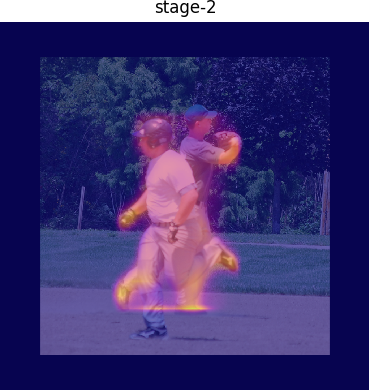
\includegraphics[height=3cm]{872_insid0_stage2.PNG}
		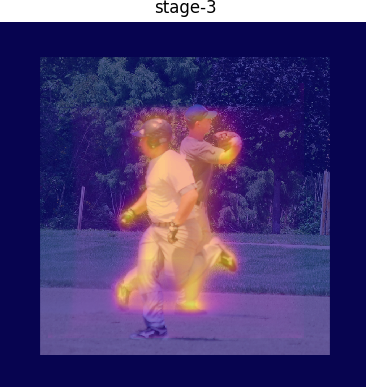
\includegraphics[height=3cm]{872_insid0_stage3.PNG}
		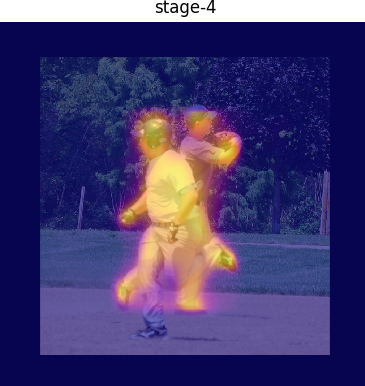
\includegraphics[height=3cm]{872_insid0_stage4.PNG}
	\end{minipage}
	\vskip0.2cm
	\begin{minipage}{\textwidth}
		遮挡
		\centering
		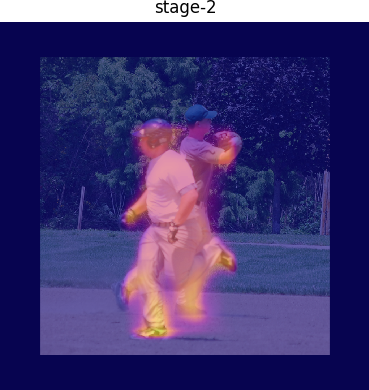
\includegraphics[height=3cm]{872_insid1_stage2.PNG}
		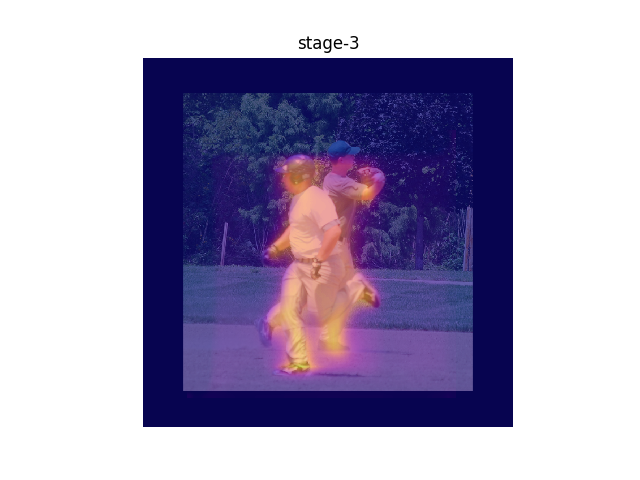
\includegraphics[height=3cm]{872_insid1_stage3.PNG}
		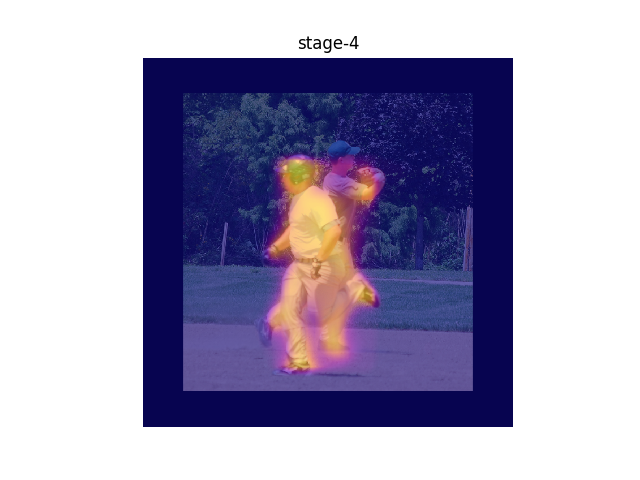
\includegraphics[height=3cm]{872_insid1_stage4.PNG}
	\end{minipage}
	\begin{minipage}{\textwidth}
		轻度遮挡
		\centering
		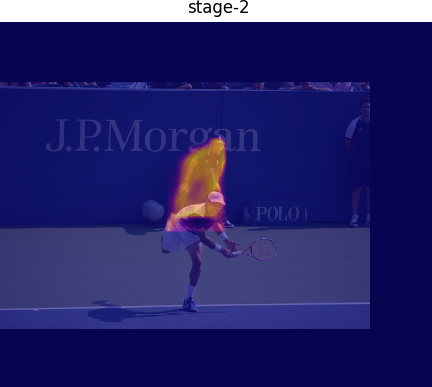
\includegraphics[height=3cm]{885_insid1_stage2.PNG}
		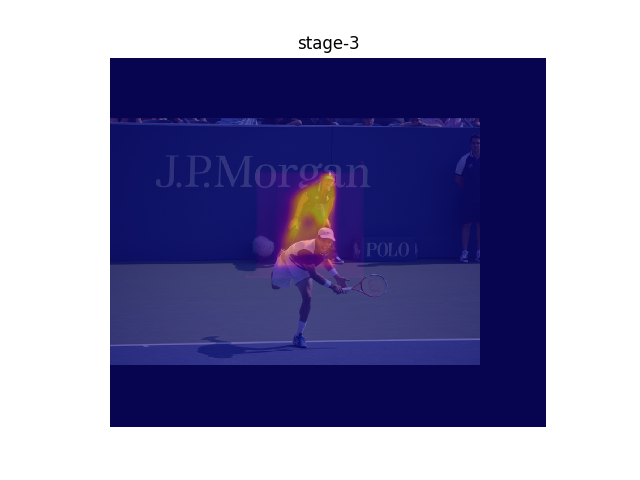
\includegraphics[height=3cm]{885_insid1_stage3.PNG}
		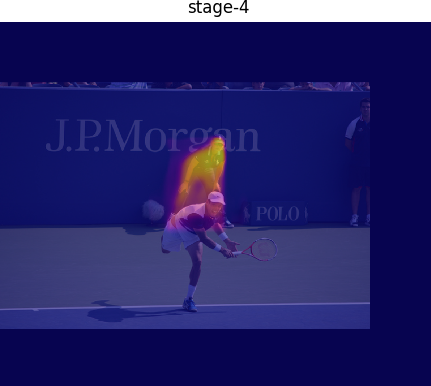
\includegraphics[height=3cm]{885_insid1_stage4.PNG}
	\end{minipage}
	\label{fig:parallel1}
	\caption{并排第一个图}
\end{figure}

\section{研究展望}
\label{sec:future}
由于时间有限,本文还有一些后续的研究展望希望在之后之后的工作中继续完善本文提出的网络结构。
\subsection{基于LSTM的注意力转移机制}
\label{subsec:lstmatten}
近年来长短时记忆(LSTM)
\subsection{基于姿态估计后目标检测}
\label{subsec:semisuperdetect}

\section{本章小结}